\subsection{ChatterBot MathBot (do FB Messenger)}\label{subsec:bot2} 
\begin{figure}[h!tbp]
    \centering
    
\includegraphics[width=0.4\linewidth]{img/bot2_logo.png}
    \caption{Avatar do perfil do MathBot (do Messenger).}
    \label{fig:bot2_logo}
\end{figure}

A proposta do Mathobot é solucionar cálculos avançados de Matemática através de uma conversa unidirecional em Inglês para usuários do aplicativo Messenger do Facebook.
Pode ser encontrado em sua página do Facebook (\url{www.facebook.com/MathChatbot})

O registro da conversa está representado abaixo:
\subsection{ChatterBot MathBot (do FB Messenger)}\label{subsec:bot2} 
\begin{figure}[h!tbp]
    \centering
    
\includegraphics[width=0.4\linewidth]{img/bot2_logo.png}
    \caption{Avatar do perfil do MathBot (do Messenger).}
    \label{fig:bot2_logo}
\end{figure}

A proposta do Mathobot é solucionar cálculos avançados de Matemática através de uma conversa unidirecional em Inglês para usuários do aplicativo Messenger do Facebook.
Pode ser encontrado em sua página do Facebook (\url{www.facebook.com/MathChatbot})

O registro da conversa está representado abaixo:
\subsection{ChatterBot MathBot (do FB Messenger)}\label{subsec:bot2} 
\begin{figure}[h!tbp]
    \centering
    
\includegraphics[width=0.4\linewidth]{img/bot2_logo.png}
    \caption{Avatar do perfil do MathBot (do Messenger).}
    \label{fig:bot2_logo}
\end{figure}

A proposta do Mathobot é solucionar cálculos avançados de Matemática através de uma conversa unidirecional em Inglês para usuários do aplicativo Messenger do Facebook.
Pode ser encontrado em sua página do Facebook (\url{www.facebook.com/MathChatbot})

O registro da conversa está representado abaixo:
\subsection{ChatterBot MathBot (do FB Messenger)}\label{subsec:bot2} 
\input{img/bot2_logo}

A proposta do Mathobot é solucionar cálculos avançados de Matemática através de uma conversa unidirecional em Inglês para usuários do aplicativo Messenger do Facebook.
Pode ser encontrado em sua página do Facebook (\url{www.facebook.com/MathChatbot})

O registro da conversa está representado abaixo:
\input{conversas/bot2}
\input{img/bot2_1}

Como se pode observar na conversa acima, o bot não consegue resolver equações.
Na realidade ele não consegue entender nem os próprios exemplos (como mostra a fig.~\ref{fig:bot2_1}).
Após um série de perguntas contendo apenas cálculos, percebi que o bot só entende e resolve problemas relacionados à aritmética e trigonometria, ou seja, funciona como uma calculadora científica básica (que geralmente são nativas em qualquer computador) e ainda com a desvantagem de ser mais lento que uma calculadora comum e ser limitada em processamento. Uma calculadora científica consegue solucionar o fatorial de $1000$ mas o MathBot não, e essa seria mais uma desvantagem.

Sugiro as seguintes melhorias para esse bot que não fogem do objetivo funcionar como uma calculadora científica:
\begin{itemize}[noitemsep]
    \item Corrigir a mensagem de ajuda, visto que essa indica problemas que o bot não soluciona
    \item Otimizar a computação dos cálculos
    \item Entender mensagens mais próximas da linguagem natural, e.g., ``sum 1 with 1''
    \item Entender alternativas de operadores, e.g., o fatorial pode ser usado como ``fact(x)'' em vez de ``$x!$''
\end{itemize}
\begin{figure}[h!tbp]
    \centering
    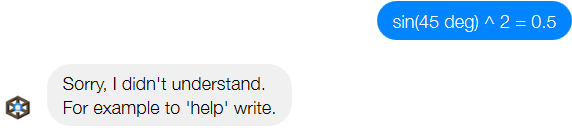
\includegraphics[width=1\linewidth]{img/bot2_1.png}
    \caption{Screenshot de uma interação com o MathBot do Messenger.}
    \label{fig:bot2_1}
\end{figure}

Como se pode observar na conversa acima, o bot não consegue resolver equações.
Na realidade ele não consegue entender nem os próprios exemplos (como mostra a fig.~\ref{fig:bot2_1}).
Após um série de perguntas contendo apenas cálculos, percebi que o bot só entende e resolve problemas relacionados à aritmética e trigonometria, ou seja, funciona como uma calculadora científica básica (que geralmente são nativas em qualquer computador) e ainda com a desvantagem de ser mais lento que uma calculadora comum e ser limitada em processamento. Uma calculadora científica consegue solucionar o fatorial de $1000$ mas o MathBot não, e essa seria mais uma desvantagem.

Sugiro as seguintes melhorias para esse bot que não fogem do objetivo funcionar como uma calculadora científica:
\begin{itemize}[noitemsep]
    \item Corrigir a mensagem de ajuda, visto que essa indica problemas que o bot não soluciona
    \item Otimizar a computação dos cálculos
    \item Entender mensagens mais próximas da linguagem natural, e.g., ``sum 1 with 1''
    \item Entender alternativas de operadores, e.g., o fatorial pode ser usado como ``fact(x)'' em vez de ``$x!$''
\end{itemize}
\begin{figure}[h!tbp]
    \centering
    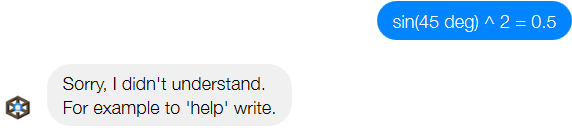
\includegraphics[width=1\linewidth]{img/bot2_1.png}
    \caption{Screenshot de uma interação com o MathBot do Messenger.}
    \label{fig:bot2_1}
\end{figure}

Como se pode observar na conversa acima, o bot não consegue resolver equações.
Na realidade ele não consegue entender nem os próprios exemplos (como mostra a fig.~\ref{fig:bot2_1}).
Após um série de perguntas contendo apenas cálculos, percebi que o bot só entende e resolve problemas relacionados à aritmética e trigonometria, ou seja, funciona como uma calculadora científica básica (que geralmente são nativas em qualquer computador) e ainda com a desvantagem de ser mais lento que uma calculadora comum e ser limitada em processamento. Uma calculadora científica consegue solucionar o fatorial de $1000$ mas o MathBot não, e essa seria mais uma desvantagem.

Sugiro as seguintes melhorias para esse bot que não fogem do objetivo funcionar como uma calculadora científica:
\begin{itemize}[noitemsep]
    \item Corrigir a mensagem de ajuda, visto que essa indica problemas que o bot não soluciona
    \item Otimizar a computação dos cálculos
    \item Entender mensagens mais próximas da linguagem natural, e.g., ``sum 1 with 1''
    \item Entender alternativas de operadores, e.g., o fatorial pode ser usado como ``fact(x)'' em vez de ``$x!$''
\end{itemize}
\begin{figure}[h!tbp]
    \centering
    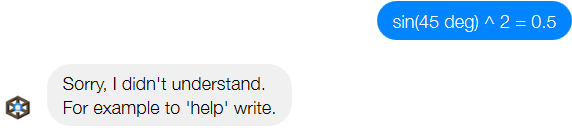
\includegraphics[width=1\linewidth]{img/bot2_1.png}
    \caption{Screenshot de uma interação com o MathBot do Messenger.}
    \label{fig:bot2_1}
\end{figure}

Como se pode observar na conversa acima, o bot não consegue resolver equações.
Na realidade ele não consegue entender nem os próprios exemplos (como mostra a fig.~\ref{fig:bot2_1}).
Após um série de perguntas contendo apenas cálculos, percebi que o bot só entende e resolve problemas relacionados à aritmética e trigonometria, ou seja, funciona como uma calculadora científica básica (que geralmente são nativas em qualquer computador) e ainda com a desvantagem de ser mais lento que uma calculadora comum e ser limitada em processamento. Uma calculadora científica consegue solucionar o fatorial de $1000$ mas o MathBot não, e essa seria mais uma desvantagem.

Sugiro as seguintes melhorias para esse bot que não fogem do objetivo funcionar como uma calculadora científica:
\begin{itemize}[noitemsep]
    \item Corrigir a mensagem de ajuda, visto que essa indica problemas que o bot não soluciona
    \item Otimizar a computação dos cálculos
    \item Entender mensagens mais próximas da linguagem natural, e.g., ``sum 1 with 1''
    \item Entender alternativas de operadores, e.g., o fatorial pode ser usado como ``fact(x)'' em vez de ``$x!$''
\end{itemize}